\begin{figure}[h]  
  \begin{center}
    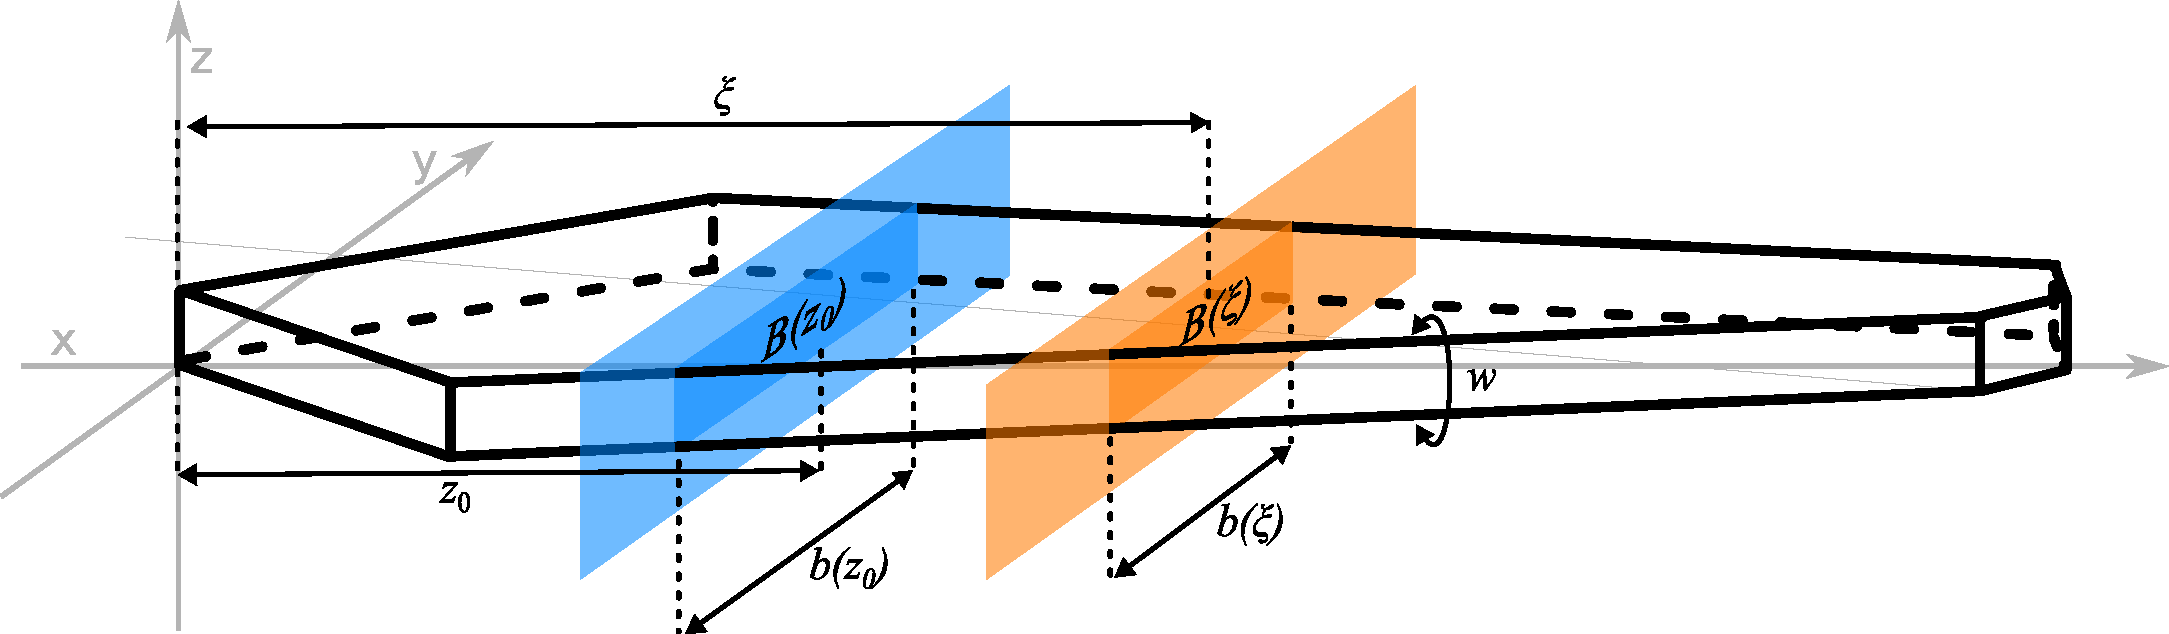
\includegraphics[width=0.95\linewidth]{./images/XiCrossSection.pdf}    
  \end{center}
  \caption[cross sections ]{Cross sections $B(ξ)$ of the channel at different positions $ξ$}
  \label{fig:XiCrossSection} 
\end{figure}
Here, the derivation is analogously conducted as described in literature \scite{Wahlund1987,Litzen1991, Wahlund2013}, 
but using the straight equations \ref{eq:chLine} for description of the channel above. This takes into consideration 
that $b(z)$ is variable over the whole channel length. In addition, also focussing into the first channel section is 
considered, for this reason, the the surface cannot just be corrected by a constant term as reported 
\scite{Litzen1991}. \tvoid is the void time of an unretained species which can be obtained by integration over the 
channel positions $ξ$.
Although this derivation leads to rather laborious expressions, it has the advantage that no additional assumptions are 
necessary. 
\begin{equation}
  \tvoid 
  = \int_0^{\tvoid}  \diff t  
  = \int_{z_0}^{L} \frac{1}{\vm(ξ)} \diff ξ 
  \label{eq:tvoidMigVelo}
\end{equation}
\vm($ξ$) is the migration velocity of the eluent at a channel position $ξ$. It dependends on the flow velocity
$\Vdot(ξ)$ at the position and the $y,z$ cross-sectional area $B(ξ)$  at (Fig \ref{fig:XiCrossSection})
\begin{equation}
  \vm(ξ) = \frac{\Vdot(ξ)}{B(ξ)} = \frac{\Vdot(ξ)}{b(ξ)\cdot w} \label{eq:MigSpeedVXi}
\end{equation}

The term $b(ξ)$ is described with the aid of eq. \ref{eq:chLine} and will require a case-by-case approach.
The change of the flow velocity $\Vdot(ξ)$ is exactly the total loss in the applied crossflow. It has its maximum at the inlet position with
\begin{equation}
  \Vdot(0) = \Vin = \Ve + \Vc
  \label{eq:DefVin}
\end{equation}
and its minimum with
\begin{equation}
  \Vdot(L) = \Ve       
\end{equation}
As this is distributed uniformly over the membrane surface, the decay is proportional to the area the eluent has already passed. This leads to the expression
\begin{equation}
  \Vdot(ξ) = \Vin - V_c \cdot \frac{A(ξ)}{\AL}    
  = \Vin - V_c \cdot \ddfrac{ \int_0^{ξ}b(x) \diff x }{ \int_0^{L}b(x) \diff x   }   
  = \Vin - V_c \cdot \ddfrac{2 \cdot \int_0^{ξ}E(x) \diff x }{ \AL  }
  \label{eq:VDepXi}
\end{equation}
The total area \AL can be easily derived by letting of eq. \ref{eq:proxFocusVolume} with letting $z_0 = 0$:
\begin{equation}
  \begin{array}{ll}
    \AL =\intGreenBox{\ensuremath{A_1}} +  \intBlueBox{\ensuremath{A_2}} + \intPurpleBox{\ensuremath{A_3}} % \left(
    &= \intGreenBox {\ensuremath{ \frac{1}{2} b_0  L_1  }}
      + \intBlueBox{\ensuremath{ \frac{1}{2} (b_0 + b_L) L_2  }}
      + \intPurpleBox{\ensuremath{ \frac{1}{2} L_3\bL  } }
      % \right)
      % \cd      
  \end{array}
  \label{eq:areaSections}
\end{equation}
To evaluate $A(ξ)$ correctly, the integrals have to be split according to the conditions in eq. \ref{eq:chLine}. This 
is required which corresponds to the cases needed for $b(ξ)$.
Merging eq. \ref{eq:tvoidMigVelo}
and \ref{eq:VDepXi} gives the expression
\begin{equation}
  \vm(ξ) = \dfrac{\Vin - V_c \cdot \frac{2 \cdot \int_0^{ξ}E(x) \diff x }{  \AL }}{ 2\cdot E(ξ) \cdot w  } 
  =\frac{1}{2\cdot w } \cdot \frac{\Vin - V_c \cdot \frac{2 \cdot \int_0^{ξ}E(x) \diff x }{ \AL }}{ E(ξ)}
\end{equation}
Inserting into eq. \ref{eq:tvoidMigVelo} gives:
\begin{equation}
  \tvoid = 2 \cdot w \cdot 
  \int_{z_0}^{L} 
  %\left(
   \ddfrac{ E(ξ) }{  \Vin - V_c \cdot \frac{2 \cdot \int_0^{ξ}E(x) \diff x }{ \AL  }  }
    %\right)
     \diff ξ
  \label{eq:awfulIntegrals}
\end{equation}
This expression quantifies a linear conversion factor $\CF$ for the relationship of  \tvoid\ and $w$. This promises a simple relationship between those two basic magnitudes with
\begin{equation}
  \tvoid = 2 \cdot \CF \cdot w
\end{equation}
and
\begin{equation}
  \CF = \int_{z_0}^{L}
  % \left(  
   \ddfrac{ E(ξ) }{ \Vin - V_c \cdot \dfrac{2 \cdot \int_0^{ξ}E(x) \diff x }{ \AL  }  
   } 
 %\right)
  \diff ξ
\end{equation}
Similar to the calculation of \Vgeo above, a case-by case analysis is required depending on $z_0$. Due to the 
section-wise definition of the integrand, the integrals then have to be split accordingly to the partial domain of 
$E(ξ)$.
\clearpage
\subsubsection*{\Vhyd: Distal focussing with $\bm{z_0 \geqq L_1}$}
  Here, the outer integral of eq. \ref{eq:awfulIntegrals} is split into the sections with  $L_1 < ξ \leqq L_{12}$ 
  and  $L_{12} < ξ$:
  % \begin{equation}
\begin{equation}
  \CF =
    \int_{z_0}^{L_{12}}  
    %\left(
      \ddfrac{ E(ξ) }{ \Vin - \frac{2V_c}{ \AL }  \int_0^{ξ}E(x) \diff x  }
     %  \right)
        \diff ξ
    +  \int_{L_{12}}^{L}
    % \left(
      \ddfrac{ E(ξ) }{ \Vin - \frac{2V_c}{ \AL  } \int_0^{ξ}E(x) \diff x  }
      % \right)
       \diff ξ 
  % \label{}
\end{equation}
As  $ξ$ is now located only on one of the section within each summand, the inner integrals can be split for the 
different domains of $E(x)$. Integrals independent from $ξ$ are directly substituted with their corresponding area 
section from eq. \ref{eq:areaSections}, only the last integral is solved.
% \end{equation}
% \begin{equation}
\begin{equation}
  \begin{array}{lllll}
    \CF &=
    &%\left( \vphantom{\ddfrac{dummy}{\int_a^b}} \right. % phantom bracket^^
    &&\displaystyle\int_{z_0}^{L_{12}}
    % \left(
       \ddfrac{  e_2(ξ)    }{   \Vin - \frac{2V_c}{ \AL  }
       \left(
       \int_0^{L_1}e_1(x) \diff x
       + \int_{L_1}^{ξ}e_2(x) \diff x
       \right)      
       }
       \diff ξ
    \\    
        &&&+& \displaystyle\int_{L_{12}}^{L}              
              \ddfrac{ e_3(ξ)  }{   \Vin - \frac{2V_c}{ \AL  }
              \left(
              \int_0^{L_1}e_1(x) \diff x
              + \int_{L_1}^{L_{12}}e_2(x) \diff x
              + \int_{L_{12}}^{ξ}e_3(x) \diff x
              \right)    
              }
              \diff ξ
              % \left.  \vphantom{\ddfrac{dummy}{\int_a^b}}   \right) %% phantom bracket^^
    \\\addlinespace[4ex]        
        &=
    &%\left( \vphantom{\ddfrac{dummy}{\int_a^b}} \right.
    &&\displaystyle\int_{z_0}^{L_{12}}
       
       \ddfrac{   m_2 \cdot ξ + t_2   }{   \Vin - \frac{2V_c}{ \AL  }
       \left(
       \frac{1}{2} A_1
       + \frac{1}{2} m_2 ( ξ^2 - L_1^2 )   + t_2( ξ - L_1 )               
       \right)
       }
       \diff ξ\\
        &&&+& \displaystyle\int_{L_{12}}^{L}
              \ddfrac{    m_3 \cdot ξ + t_3  }{   \Vin - \frac{2V_c}{ \AL  }
              \left(
              \frac{1}{2} A_1
              + \frac{1}{2} A_2 
              + \frac{1}{2} m_3 ( ξ^2 - L_{12}^2 )   + t_3( ξ - L_{12} )          
              \right)             
              }
              \diff ξ
              % \left. \vphantom{\ddfrac{dummy}{\int_a^b}}  \right) %% phantom bracket^^
    \\
  \end{array}
  % \label{}
\end{equation}
In order to transform the integrand terms into ordinary rational functions and simplify the analytical solutions 
This can be rearranged by using substitutions for the occurring prefactors $α_i,β_i,γ_i,δ_i$, the quadratic polynomials 
$P(ξ)$ and its discriminants
$Δ_i$:
\begin{equation}
  \begin{array}{lllll}
    α_2 = \frac{t_2}{m_2}
    & β_2 = -\frac{\Vc m_2}{ \AL }
    & γ_2 = -\frac{2 \Vc t_2}{\AL}\\\addlinespace
    \multicolumn{3}{l}{ δ_2 = \Vin - \frac{\Vc}{\AL} \left( A_1 - m_2L_1^2 - 2t_2L_1  \right) }
    & Δ_2 =4β_2 δ_2 - γ_2^2
    \\\addlinespace[2ex]
    α_3 = \frac{t_3}{m_3}
    &β_3 = -\frac{\Vc m_3}{ \AL }
    &γ_3 = -\frac{2 \Vc t_3}{\AL}\\\addlinespace
    \multicolumn{3}{l}{ δ_3 =\Vin - \frac{\Vc}{\AL} \left( A_1 + A_2 - m_3L_{12}^2 - 2t_3L_{12}  \right) }
    & Δ_3 =  4β_3 δ_3 - γ_3^2
  \end{array}%{lllllllll}
\end{equation}
\begin{equation}
  \begin{array}{ll}
    P_2(ξ) = β_2 ξ^2 + γ_2 ξ + \delta_2\\\addlinespace[2ex]
    P_3(ξ) = β_3 ξ^2 + γ_3 ξ + \delta_3
  \end{array}
\end{equation}
  For solving the integral it is important to know the sign of $\Delta_2$ and $\Delta_3$. Inserting \ref{eq:DefVin}, it 
  can be shown (see below) that it is not possible to determine the scope of $\Delta_2$ exactly for the general case 
  and the case-by-case analysis has to be conducted ``at runtime''. To simplify the display of this expression, it 
  is split and each summand treated separately:
      \begin{equation}
  \CF = \CFtwo +\CFthree  
\end{equation}
\begin{equation}
  \begin{array}{lllll}
    \CFtwo &= 
    &   m_2 \cdot \displaystyle\int_{z_0}^{L_{12}}  
      \ddfrac{    ξ + α_2   }{
      β_2 ξ^2 + γ_2 ξ + \delta_2
      }
      \diff ξ \\\addlinespace
      %%%%%%%%%%%%%%%%%%%%% 
           &= 
    &   m_2 \cdot
      \left(
      \displaystyle\int_{z_0}^{L_{12}}       
      \ddfrac{ ξ }{
      P_2(ξ) % β_2 ξ^2 + γ_2 ξ + \delta_2
      }
      \diff ξ
      +
      \displaystyle\int_{z_0}^{L_{12}}       
      \ddfrac{ α_2 }{
      P_2(ξ) % β_2 ξ^2 + γ_2 ξ + \delta_2
      }
      \diff ξ
      \right)     \\\addlinespace
      %%%%%%%%%%%%%%%%%%%%%%% 
           &=
    &m_2 \cdot
      \left(
      \left[    \frac{\ln{P_2(ξ)}}{2β_2} \right]_{z_0}^{L_{12}}

      + 
      \left(
      α_2 - \frac{γ_2}{2β_2}
      \right)
      \displaystyle\int_{z_0}^{L_{12}}       
      \ddfrac{\diff ξ }{
      P_2(ξ) % β_2 ξ^2 + γ_2 ξ + \delta_2
      }             
      \right) & \scite{Bronstein2008}
    \\\addlinespace
           &=
    &\begin{cases}
      %%%%%%%%%%%%%%%%%%%%%%% 
      \mathrlap{
        m_2 \cdot
        \left(
          \left[ \frac{\ln{P_2(ξ)}}{2β_2} \right]_{z_0}^{L_{12}}
          + 
          \left(
            α_2 - \frac{γ_2}{2β_2}
          \right)
          \left[
            \ddfrac{2}{\sqrt{Δ_2}} \cdot \text{arctan}{\left( \ddfrac{ \displaystyle 2β_2\xi+γ_2 }{\displaystyle 
            \sqrt{Δ_2} } \right) }
          \right]_{z_0}^{L_{12}}
        \right)
      }
      \phantom{      m_2 \cdot \left(\frac{1}{2β_2}\ln{\frac{P_2(L_{12})}{ P_2(z_0)}}-\left(\frac{2}{\sqrt{-Δ_2}}\right)\left(α_2 - \frac{γ_2}{2β_2}\right)\left(\text{artanh}\ddfrac{2β_2 (L_{12} - z_0)}{\left(\sqrt{-Δ_2}- \scriptstyle
                \frac{ \left(2β_2L_{12}+γ_2 \right)  \left(2β_2z_0+γ_2 \right) }{\sqrt{-Δ_2}}\right)}\right)\right)                  }    
      & \forall Δ_2 > 0
      \\\addlinespace
      m_2 \cdot
      \left(
        \left[ \frac{\ln{P_2(ξ)}}{2β_2} \right]_{z_0}^{L_{12}}
        + 
        \left(
          α_2 - \frac{γ_2}{2β_2}
        \right)
        \left[
          -\ddfrac{2}{\sqrt{-Δ_2}} \cdot \text{artanh}{\left( \ddfrac{ 2β_2\xi+γ_2 }{ \sqrt{-Δ_2} } \right) }
        \right]_{z_0}^{L_{12}} 
      \right) & \forall Δ_2 < 0 \\\addlinespace
    \end{cases} & \scite{Bronstein2008a}
    %%%%%%%%%% 
    \\\addlinespace
           &=
    &\begin{cases}
      \mathrlap{
        m_2 \cdot \Bigg(
        \frac{1}{2β_2}
        \Big(\scriptstyle
        \ln{P_2(L_{12})} - \ln{P_2({z_0})}
        \Big)
        +
        \left(
          \frac{2}{\sqrt{Δ_2}}
        \right)
        \left(
          α_2 - \frac{γ_2}{2β_2}
        \right)
        \left(
          \text{arctan} \ddfrac{ 2β_2L_{12}+γ_2 }{ \sqrt{Δ_2} }
          - \text{arctan} \ddfrac{ 2β_2z_0+γ_2 }{ \sqrt{Δ_2} }
        \right)        
        \Bigg)
      }
      \phantom{      m_2 \cdot \left(\frac{1}{2β_2}\ln{\frac{P_2(L_{12})}{ P_2(z_0)}}-\left(\frac{2}{\sqrt{-Δ_2}}\right)\left(α_2 - \frac{γ_2}{2β_2}\right)\left(\text{artanh}\ddfrac{2β_2 (L_{12} - z_0)}{\left(\sqrt{-Δ_2}- \scriptstyle
                \frac{ \left(2β_2L_{12}+γ_2 \right)  \left(2β_2z_0+γ_2 \right) }{\sqrt{-Δ_2}}\right)}\right)\right)                  }
      & \forall Δ_2 > 0\\\addlinespace
      m_2 \cdot \Bigg(
      % \left(
      \frac{1}{2β_2}
      \Big(\scriptstyle
      \ln{P_2(L_{12})} - \ln{P_2({z_0})}
      \Big)
      -
      \left(
        \frac{2}{\sqrt{-Δ_2}}
      \right)
      \left(
        α_2 - \frac{γ_2}{2β_2}
      \right)
      \left(
        \text{artanh} \ddfrac{ 2β_2L_{12}+γ_2 }{ \sqrt{-Δ_2} }
        - \text{artanh} \ddfrac{ 2β_2z_0+γ_2 }{ \sqrt{-Δ_2} }
      \right)
      % \right)
      \Bigg) & \forall Δ_2 < 0 
    \end{cases} 
    %%%%%%%%%% 
    \\\addlinespace
           &=
    &\begin{cases}
      \mathrlap{
        m_2 \cdot \left(
          \frac{1}{2β_2}       
          \ln{\frac{P_2(L_{12})}{ P_2(z_0)}}
          +
          \left(
            \frac{2}{\sqrt{Δ_2}}
          \right)
          \left(
            α_2 - \frac{γ_2}{2β_2}
                \right)
            \left(
              \text{arctan} \ddfrac{ 2β_2L_{12}+γ_2 }{ \sqrt{Δ_2} }
              - \text{arctan} \ddfrac{ 2β_2z_0+γ_2 }{ \sqrt{Δ_2} }            
          \right)
        \right)
      }\phantom{      m_2 \cdot \left(\frac{1}{2β_2}\ln{\frac{P_2(L_{12})}{ P_2(z_0)}}-\left(\frac{2}{\sqrt{-Δ_2}}\right)\left(α_2 - \frac{γ_2}{2β_2}\right)\left(\text{artanh}\ddfrac{2β_2 (L_{12} - z_0)}{\left(\sqrt{-Δ_2}- \scriptstyle
                \frac{ \left(2β_2L_{12}+γ_2 \right)  \left(2β_2z_0+γ_2 \right) }{\sqrt{-Δ_2}}\right)}\right)\right)                  }    
      & \forall Δ_2 > 0
      \\\addlinespace
      m_2 \cdot \left(
        \frac{1}{2β_2}       
        \ln{\frac{P_2(L_{12})}{ P_2(z_0)}}
        -
        \left(
          \frac{2}{\sqrt{-Δ_2}}
        \right)
        \left(
          α_2 - \frac{γ_2}{2β_2}
        \right)
        \left(          
          \text{artanh}
          \frac{2β_2L_{12}+ γ_2 - 2β_2z_0-γ_2
          }{
            \sqrt{-Δ_2} \cdot \left(
              1 - \scriptstyle
              \frac{2β_2L_{12}+γ_2 }{ \sqrt{-Δ_2} } \cdot
              \frac{2β_2z_0+γ_2 }{ \sqrt{-Δ_2} }
            \right)

          }
        \right)        
      \right)
      & \forall Δ_2 < 0 
    \end{cases}
    \\\addlinespace
    %%%%%%%%%%%%%%%%%%% 
           &= &\begin{cases}
             m_2 \cdot \left(
               \frac{1}{2β_2}       
               \ln{\frac{P_2(L_{12})}{ P_2(z_0)}}
               +
               \left(
                 \frac{2}{\sqrt{Δ_2}}
               \right)
               \left(
                 α_2 - \frac{γ_2}{2β_2}
                  \right) 
                 \left(
                   \text{arctan} \ddfrac{ 2β_2L_{12}+γ_2 }{ \sqrt{Δ_2} }
                   - \text{arctan} \ddfrac{ 2β_2z_0+γ_2 }{ \sqrt{Δ_2} }                   
               \right)
             \right)
             & \forall Δ_2 > 0\\\addlinespace
             m_2 \cdot \left(
               \frac{1}{2β_2}       
               \ln{\frac{P_2(L_{12})}{ P_2(z_0)}}
               -
               \left(
                 \frac{2}{\sqrt{-Δ_2}}
               \right)
               \left(
                 α_2 - \frac{γ_2}{2β_2}
               \right)
               \left(
                 \text{artanh}
                 \ddfrac{2β_2 (L_{12} - z_0)
                 }{
                   \left(
                     \sqrt{-Δ_2}- \scriptstyle
                     % \frac{2β_2L_{12}+γ_2 }{ \sqrt{-Δ_2} } \cdot
                     \frac{ \left(2β_2L_{12}+γ_2 \right)  \left(2β_2z_0+γ_2 \right) }{\sqrt{-Δ_2}}
                     % \frac{2β_2z_0+γ_2 }{ \sqrt{-Δ_2} }
                   \right)
                 }
               \right)        
             \right)    & \forall Δ_2 < 0 
           \end{cases}                
  \end{array}    \label{eq:CFtwo}  
\end{equation}

\begin{equation}
  \begin{array}{lclll}
    \CFthree &=
    & m_3 \cdot \displaystyle\int_{L_{12}}^{L}
      \ddfrac{   ξ + α_3
      }{
      β_3 ξ^2 + γ_3 ξ + \delta_3
      }
      \diff ξ \\\addlinespace
             & =&  m_3 \cdot
                  \left(
                  \displaystyle\int_{L_{12}}^{L}       
                  \ddfrac{ ξ }{
                  P_3(ξ) % β_2 ξ^2 + γ_2 ξ + \delta_2
                  }
                  \diff ξ
                  +
                  \displaystyle\int_{L_{12}}^{L}       
                  \ddfrac{ α_3 }{
                  P_3(ξ) % β_2 ξ^2 + γ_2 ξ + \delta_2
                  }
                  \diff ξ
                  \right)
                  % \right)
    \\\addlinespace[2ex]
             &&    \cdots\ \text{analogously to eq. \ref{eq:CFtwo} }\cdots    \\\addlinespace[2ex]
             &=
    & \begin{cases}
      m_3 \cdot \left(
        \frac{1}{2β_3}       
        \ln{\frac{P_3(L)}{ P_3(L_{12})}}
        +
        \left(
          \frac{2}{\sqrt{Δ_3}}
        \right)
        \left(
          α_3 - \frac{γ_3}{2β_3}
           \right)  
          \left(
            \text{arctan} \ddfrac{ 2β_3L+γ_3 }{ \sqrt{Δ_3} }
            - \text{arctan} \ddfrac{ 2β_3L_{12}+γ_3 }{ \sqrt{Δ_3} }           
        \right)
      \right)
      & \forall Δ_3 > 0\\\addlinespace
      m_3 \cdot \left(
        \frac{1}{2β_3}       
        \ln{\frac{P_3(L)}{ P_3(L_{12})}}
        -
        \left(
          \frac{2}{\sqrt{-Δ_3}}
        \right)
        \left(
          α_3 - \frac{γ_3}{2β_3}
        \right)
        \left(
          \text{artanh}
          \ddfrac{2β_3 (L - L_{12})
          }{
            \left(
              \sqrt{-Δ_3}- \scriptstyle
              % \frac{2β_2L_{12}+γ_2 }{ \sqrt{-Δ_2} } \cdot
              \frac{ \left(2β_3L+γ_3 \right)  \left(2β_3L_{12}+γ_3 \right) }{\sqrt{-Δ_3}}
              % \frac{2β_2z_0+γ_2 }{ \sqrt{-Δ_2} }
            \right)

          }
        \right)        
      \right)    & \forall Δ_3 < 0
      %%%%%%%%%%%%%%%%%%%%%       
    \end{cases}
  \\\addlinespace[2ex]
             &=
    & \begin{cases}
      m_3 \cdot \left(
        \frac{1}{2β_3}
        \ln{\frac{P_3(L)}{ P_3(L_{12})}}
        +
        \left(
          \frac{2}{\sqrt{Δ_3}}
        \right)
        \left(
          α_3 - \frac{γ_3}{2β_3}
          \right) 
          \left(
            \text{arctan} \ddfrac{ 2β_3L+γ_3 }{ \sqrt{Δ_3} }
            - \text{arctan} \ddfrac{ 2β_3L_{12}+γ_3 }{ \sqrt{Δ_3} }             
        \right)
      \right)
      & \forall Δ_3 > 0\\\addlinespace
      m_3 \cdot \left(
        \frac{1}{2β_3}       
        \ln{\frac{P_3(L)}{ P_3(L_{12})}}
        -
        \left(
          \frac{2}{\sqrt{-Δ_3}}
        \right)
        \left(
          α_3 - \frac{γ_3}{2β_3}
        \right)
        \left(
          \text{artanh}
          \ddfrac{2β_3\left( L- L_{12} \right)
          }{
            \left(
              \sqrt{-Δ_3}- \scriptstyle
              % \frac{2β_2L_{12}+γ_2 }{ \sqrt{-Δ_2} } \cdot
              \frac{ \left(2β_3L+γ_3 \right)  \left(2β_3L_{12}+γ_3 \right) }{\sqrt{-Δ_3}}
              % \frac{2β_2z_0+γ_2 }{ \sqrt{-Δ_2} }
            \right)            
          }
        \right)        
      \right)    & \forall Δ_3 < 0
    \end{cases}
  \end{array}
\end{equation}
\clearpage
% The last expression can be easily evaluated and needs only to call 6 numerical subroutines (which would be relevant if it was embedded into an algorithm with numerous calls of this calculation).
\subsubsection*{\Vhyd: Proximal focusing with $\bm{z_0 < L_1}$}
If the sample was focused to a point with $z_0 < L_1$, the in addition to the solution above, also the eluent migration 
through the first sections has to be considered. The evaluation of the expression can be conducted analogously for the 
second and third summand as shown above with adaption of the lower limit of integration for the second:
\begin{equation}
  \begin{array}{lcll}
    \CF
    &=      
    &     % \left(% \vphantom{\ddfrac{dummy}{\int_a^b}} \right.
    &\displaystyle\int_{z_0}^{L_{1}}  \ddfrac{  e_1(ξ)  }{   \Vin - \frac{2V_c}{ \AL  }
      \left(
      \int_0^{ξ}e_1(x) \diff x
      \right)
      }  \diff ξ\\
    &&+&  \displaystyle\int_{L_1}^{L_{12}}    \ddfrac{  e_2(ξ)  }{   \Vin - \frac{2V_c}{ \AL  }
         \left(
         \int_0^{L_1}e_1(x) \diff x
         + \int_{L_1}^{ξ}e_2(x) \diff x
         \right) }
         \diff ξ\\
    &&+& \displaystyle\int_{L_{12}}^{L} %\left(
         \ddfrac{   e_3(ξ)  }{   \Vin - \frac{2V_c}{ \AL  }
         \left(
         \int_0^{L_1}e_1(x) \diff x
         + \int_{L_1}^{L_{12}}e_2(x) \diff x
         + \int_{L_{12}}^{ξ}e_3(x) \diff x
         \right)    }
         \diff ξ
         % \left. \vphantom{\ddfrac{dummy}{\int_a^b}}          \right)%% phantom bracket^^
    \\   
    &=      
    &%2 \cdot w \cdot
    % \left(
    %   \vphantom{\ddfrac{dummy}{\int_a^b}} \right.
    &\displaystyle\int_{z_0}^{L_{1}}  \ddfrac{  m_1 \cdot ξ  }{   \Vin - \frac{2V_c}{ \AL  }
      \left(
      \frac{1}{2} m_1 ξ^2  
      \right)
      } \diff ξ\\
    &&+&  \displaystyle\int_{L_1}^{L_{12}}    \ddfrac{ m_2 \cdot ξ + t_2 }{   \Vin - \frac{2V_c}{ \AL  }
         \left(
         \frac{1}{2} A_1
         + \frac{1}{2} m_2 ( ξ^2 - L_1^2 )   + t_2( ξ - L_1 ) 
         \right)
         } \diff ξ\\
    &&+& \displaystyle\int_{L_{12}}^{L}  \ddfrac{  m_3 \cdot ξ + t_3   }{   \Vin - \frac{2V_c}{ \AL  }
         \left(
         \frac{1}{2} A_1 
         + \frac{1}{2} A_2    
         + \frac{1}{2} m_3 ( ξ^2 - L_{12}^2 )   + t_3( ξ - L_{12} )   
         \right)    
         } \diff ξ
         % \left. \vphantom{\ddfrac{dummy}{\int_a^b}}  \right)%% phantom bracket^^
    \\
  \end{array}
\end{equation}

Substitution is done similarly as above:
\begin{equation}  
  \begin{array}{lllll}
    & β_1 = -\frac{\Vc m_1}{ \AL }
    & δ_1 = \Vin   %\frac{2 \Vc t_1}{\AL}
    \\\addlinespace
    α_2 = \frac{t_2}{m_2}
    & β_2 = -\frac{\Vc m_2}{ \AL }
    & γ_2 = -\frac{2 \Vc t_2}{\AL}\\\addlinespace
    \multicolumn{3}{l}{ δ_2 = \Vin - \frac{\Vc}{\AL} \left( A_1 - m_2L_1^2 - 2t_2L_1  \right) }
    & Δ_2 =4β_2 δ_2 - γ_2^2
    \\\addlinespace[2ex]
    α_3 = \frac{t_3}{m_3}
    &β_3 = -\frac{\Vc m_3}{ \AL }
    &γ_3 = -\frac{2 \Vc t_3}{\AL}\\\addlinespace
    \multicolumn{3}{l}{ δ_3 =\Vin - \frac{\Vc}{\AL} \left( A_1 + A_2 - m_3L_{12}^2 - 2t_3L_{12}  \right) }
    & Δ_3 =  4β_3 δ_3 - γ_3^2
  \end{array}%{lllllllll}
\end{equation}
\begin{equation}
  \begin{array}{ll}
    P_2(ξ) = β_2 ξ^2 + γ_2 ξ + \delta_2\\\addlinespace[2ex]
    P_3(ξ) = β_3 ξ^2 + γ_3 ξ + \delta_3
  \end{array}
\end{equation}
\clearpage
Then, in analogy, to the case $z_0 \geqq L_1$, $\CF$ can be expressed as 
\begin{equation}
  \begin{array}{lcll}
    \CF  &= &\CFone + \CFtwo + \CFthree\\
         & =    
            &&       
       m_1 \cdot \displaystyle\int_{z_0}^{L_{1}}
       \left(
       \ddfrac{
       ξ 
       }{
       β_1 \cdot ξ^2 + δ_1
       } \right) \diff ξ
    \\\addlinespace
        &&+& m_2 \cdot \displaystyle\int_{L_1}^{L_{12}} \left(
             \ddfrac{
             ξ + α_2         
             }{
             β_2 ξ^2 + γ_2 ξ + δ_2          
             } \right) \diff ξ
    \\\addlinespace
        &&+& m_3 \cdot \displaystyle\int_{L_{12}}^{L} \left(
             \ddfrac{
             ξ + α_3        
             }{
             β_3 ξ^2 + γ_3 ξ + δ_3 
             } \right) \diff ξ
  \end{array}
  % \label{}
\end{equation}
with
%%%% CF1
\begin{equation}
  \begin{array}{lcll}
    \CFone &=
    & m_1 \cdot \displaystyle\int_{z_0}^{L_{1}}
      \left(
      \ddfrac{
      ξ 
      }{
      β_1 \cdot ξ^2 + δ_1
      } \right) \diff ξ
    \\ \addlinespace[1ex]
    &= & \frac{ m_1}{ β_1} \cdot \displaystyle\int_{z_0}^{L_{1}}
    \left(
    \frac{
    ξ 
    }{
    \scriptstyle \frac{δ_1}{β_1} + \displaystyle ξ^2 W 
  } \right) \diff ξ
  \\ \addlinespace[1ex]
     &= &\ddfrac{ m_1}{ β_1} \cdot \frac{1}{2}
     \left[
       \ln(\left| \ddfrac{δ_1}{β_1} + \displaystyle ξ^2 \right|)
     \right]_{z_0}^{L_{1}} %& \scite{Bronstein2008b}
   \\ \addlinespace[1ex]
  &= &\ddfrac{ m_1}{2 β_1} \cdot 
    \left(
      \ln \left| \ddfrac{δ_1}{β_1} + \displaystyle L_1^2 \right| 
      -
      \ln \left| \ddfrac{δ_1}{β_1} + \displaystyle z_0^2 \right| 
    \right)
  \end{array}
  % \label{}
\end{equation}
%%%% CF2
\begin{equation}
  \begin{array}{lclll}
    \CFtwo &= &\begin{cases}
      m_2 \cdot \left(
        \frac{1}{2β_2}       
        \ln{\frac{P_2(L_{12})}{ P_2(L_1)}}
        +
        \left(
          \frac{2}{\sqrt{Δ_2}}
        \right)
        \left(
          α_2 - \frac{γ_2}{2β_2}
       \right)    
          \left(
            \text{arctan} \ddfrac{ 2β_2L_{12}+γ_2 }{ \sqrt{Δ_2} }
            - \text{arctan} \ddfrac{ 2β_2L_1+γ_2 }{ \sqrt{Δ_2} }
        \right)
      \right)
             & \forall Δ_2 > 0\\\addlinespace
             m_2 \cdot \left(
               \frac{1}{2β_2}       
               \ln{\frac{P_2(L_{12})}{ P_2(L_1)}}
               -\left(
                 \frac{2}{\sqrt{-Δ_2}}
               \right)
               \left(
                 α_2 - \frac{γ_2}{2β_2}
               \right)
               \left(
                 \text{artanh}
                 \ddfrac{2β_2 (L_{12} - L_1)
                 }{
                   \left(
                     \sqrt{-Δ_2}- \scriptstyle
                     % \frac{2β_2L_{12}+γ_2 }{ \sqrt{-Δ_2} } \cdot
                     \frac{ \left(2β_2L_{12}+γ_2 \right)  \left(2β_2z_0+γ_2 \right) }{\sqrt{-Δ_2}}
                     % \frac{2β_2z_0+γ_2 }{ \sqrt{-Δ_2} }
                   \right)                   
                 }
               \right)        
             \right)    & \forall Δ_2 < 0 
           \end{cases}                
  \end{array}
\end{equation}


%%%% CF3

\begin{equation}
  \begin{array}{lclll}
    \CFthree &=    & \begin{cases}
      m_3 \cdot \left(
        \frac{1}{2β_3}       
        \ln{\frac{P_3(L)}{ P_3(L_{12})}}
        +
        \left(
          \frac{2}{\sqrt{Δ_3}}
        \right)
        \left(
          α_3 - \frac{γ_3}{2β_3}
           \right)
          \left(
            \text{arctan} \ddfrac{ 2β_3L+γ_3 }{ \sqrt{Δ_3} }
            - \text{arctan} \ddfrac{ 2β_3L_{12}+γ_3 }{ \sqrt{Δ_3} }             
        \right)
      \right)
      & \forall Δ_3 > 0\\\addlinespace
      m_3 \cdot \left(
        \frac{1}{2β_3}       
        \ln{\frac{P_3(L)}{ P_3(L_{12})}}
        -\left(
          \frac{2}{\sqrt{-Δ_3}}
        \right)
        \left(
          α_3 - \frac{γ_3}{2β_3}
        \right)
        \left(
          \text{artanh}
          \ddfrac{2β_3\left( L- L_{12} \right)
          }{
            \left(
              \sqrt{-Δ_3}- \scriptstyle
              % \frac{2β_2L_{12}+γ_2 }{ \sqrt{-Δ_2} } \cdot
              \frac{ \left(2β_3L+γ_3 \right)  \left(2β_3L_{12}+γ_3 \right) }{\sqrt{-Δ_3}}
              % \frac{2β_2z_0+γ_2 }{ \sqrt{-Δ_2} }
            \right)            
          }
        \right)        
      \right)    & \forall Δ_3 < 0
    \end{cases}
  \end{array}
  % \label{}
\end{equation}
                                                           
 \subsubsection*{Evaluation of $\bm \Delta_2$}
To avoid an additional case-by-case analysis for the integration, the discriminants the polynomials $P_2(ξ)$ and $P_3(ξ)$ each were resubsituted to derive that only one of the cases
\[
  \int \frac{\diff ξ}{β_i ξ^2 + γ_i ξ + δ_i}
  \left\{  
    \begin{array}{llll}
      = \ddfrac{2}{\sqrt{Δ_i}} \cdot \arctan{\left( \ddfrac{ 2β_iξ_i+γ_i }{ \sqrt{Δ_i} } \right) }
      & \forall &  Δ_i > 0  \\\addlinespace %\label{eq:chLine1} \\
      = - \ddfrac{2}{\sqrt{-Δ_i}} \cdot \text{artanh}{\left( \ddfrac{ 2β_iξ_i+γ_i }{ \sqrt{-Δ_i} } \right)}
      & \forall & Δ_i < 0  \\ %  \label{eq:chLine3}
    \end{array}
  \right. \qquad\ \scite{Bronstein2008a}
  % \label{eq:chLine}
  % end{align}  
\]
has to be applied for the evaluation of $\CF$:\clearpage
%%%%%%%%%%%%%%%%%%%%%%%%% 
%\vspace*{2ex}\\
%$\bm{z_0 \geqq L_1}$\\
\begin{equation}
  \begin{array}{lll}
    Δ_2
    &=  4β_2δ_2 - γ_2^2      
    \\\addlinespace
    &= 
      4 \cdot \left(- \frac{\Vc m_2}{\AL} \right) \cdot
      \left(
      \Vin - \frac{\Vc}{\AL} \left(  A_1 - m_2L_1^2 - 2t_2L_1 \right)
      \right)
      -\left( - \frac{2 \Vc t_2}{\AL} \right)^2
    \\\addlinespace
    &=     
      - 4 \cdot \frac{\Vc m_2 \Vin}{\AL}
      + 4\cdot \frac{\Vc^2m_2A_1}{\AL^2}
      - 4\cdot \frac{\Vc^2m_2^2L_1^2}{\AL^2}
      - 4\cdot \frac{2 \Vc^2m_2 t_2 L_1}{\AL^2}
      - 4 \cdot \frac{\Vc^2t_2^2}{\AL^2}
    \\\addlinespace   
    &=
      \left( 4 \cdot \frac{\Vc^2}{\AL^2} \right)
      \cdot \left(- m_2A_1 + m_2^2L_1^2 - 2 m_2t_2L_1 -t_2^2  \right)      
      - 4 \cdot \frac{\Vc m_2 \Vin}{\AL}
    \\\addlinespace
    &=
      \left( \frac{\Vc^2}{\AL^2} \right)
      \cdot \left(
      -   \frac{L_1}{L_2} b_0\bDelta 
      - \markOrange{   \frac{L_1^2}{L_2^2}b_\Delta^2 }
      + \markBlue{ 2 \frac{L_1}{L_2}  b_0\bDelta }
      + \markOrange{2 \frac{L_1^2}{L_2^2}\bDelta^2}
      - b_0^2
      - \markBlue{ 2 \frac{L_1}{L_2}b_0\bDelta}
      -\markOrange{ \frac{L_1^2}{L_2^2}b_\Delta^2}
      \right) 
      % - 4 \cdot \frac{\Vc^2t_2^2}{\AL^2}
      +  2 \cdot \frac{\bDelta \Vc \Vin}{L_2 \AL}
    \\\addlinespace 
    % \renewcommand{\phantItem}{\left( \frac{\Vc^2}{\AL^2} \right) }
    &=
    % \underbrace{\vphantom{\phantItem}
      \left( \frac{\Vc^2}{\AL^2} \right)
      % }_{>0}
      \cdot \left(      
        % \underbrace{\vphantom{\left( \frac{\Vc^2}{\AL^2} \right) }
      -   \frac{L_1}{L_2}  b_0\bDelta   %  }_{<0}
      % \underbrace{\vphantom{\left( \frac{\Vc^2}{\AL^2} \right) }
      % -\markOrange{2 \frac{L_1^2}{L_2^2}\bDelta^2}}_{<0}
      % \underbrace{\vphantom{\left( \frac{\Vc^2}{\AL^2} \right) }
      - b_0^2
      %%%%% }_{<0}
      \right)
      % \underbrace{\vphantom{\left( \frac{\Vc^2}{\AL^2} \right) }
      + 2 \cdot \frac{\bDelta \Vc \Vin}{L_2 \AL}      
      % }_{<0\ \text{with}\ m_2<0}
      %   \renewcommand{\phantItem}{}

    \\\addlinespace
    &=    
      \left( \frac{\Vc}{\AL} \right)    
      \cdot \left(

      -  \frac{\Vc}{\AL}  \frac{L_1}{L_2}  b_0\bDelta        
      -          \frac{\Vc}{\AL} b_0^2         
      + 2  \frac{\bDelta}{L_2}  \Vin        
      \right)    
      
    \\\addlinespace
    &=   \left( \frac{\Vc}{\AL^2} \right)     
      \left(       
      \Vin  \cdot  \left(
      2 \frac{\bDelta}{L_2} \AL
      \right)
      - \Vc
      \cdot \left(      
      \frac{L_1}{L_2}  b_0\bDelta        
      + b_0^2                   
      \right)     
      \right)      
    \\\addlinespace
    &=
      \left( \frac{\Vc}{\AL^2} \right)     
      \left(       
      \Vin  \cdot  \left(
      2 \frac{\bDelta}{L_2}
      \left(
      \frac{1}{2} b_0  L_1 
      +  \frac{1}{2} (b_0 + b_L) L_2 
      + \frac{1}{2} L_3\bL        
      \right)      
      \right)
      - \Vc
      \cdot \left(      
      \frac{L_1}{L_2}  b_0\bDelta        
      + b_0^2                   
      \right)     
      \right)
      %%%% DEBUGGED UNTIL HERE
    \\\addlinespace
    &=
      \left( \frac{\Vc}{\AL^2} \right)     
      \left(       
      \Vin  \cdot  \left(
      \frac{L_1 }{L_2} \bDelta b_0
      + \bDelta b_0
      + \bDelta b_L
      + \frac{L_3}{L_2} b_L \bDelta
      \right)          
      - \Vc
      \cdot \left(      
      \frac{L_1}{L_2}  b_0\bDelta        
      + b_0^2                   
      \right)
      \right)
      %%%% DEBUGGED UNTIL HERE
  \end{array}
\end{equation}
It turns out that the sign of the discriminant cannot be determined exactly without prior knowledge about the 
parameters. and the sign of the discriminants have to be determined ``at runtime''.